\clearpage
\twocolumn[{%
\subsection{Decision accuracy on decisive pairs}
\label{app:rq02_decisive_pairs}

\noindent\begin{minipage}[t]{0.485\textwidth}
\vspace{0pt}
\paragraph{Research Question.} \emph{Does a proxy rank the design decisions better once the pairs the 1.7B reference itself cannot separate from seed noise are left out?}

\paragraph{Setup.} Seed-1904 runs of every language setting, ladder and data build, 90M--1.7B, on pairs that may differ on any number of design axes. A pair is decisive for a task when its gap at 1.7B exceeds $k \sqrt{2}$ times the task's seed standard deviation, for $k \in \{1, 2\}$. The seed standard deviation is the median, over the baseline cells trained with three seeds (175M, 600M and 1B), of the standard deviation of the final score. There are no replicates at 1.7B, so we assume that seed noise does not grow with size. Every line reads the same accuracy tasks: those with a seed standard deviation and at least three pairs above the larger threshold, above chance at the proxy and at 1.7B.
\end{minipage}\hfill
\begin{minipage}[t]{0.485\textwidth}
\vspace{0pt}
\begin{rqfinding}
\textbf{1. Benchmark DA rises on decisive pairs.} On the same 206--303 tasks, multi-axis DA-size goes from 0.55--0.58 on every pair to 0.61--0.65 above one seed sd and 0.67--0.72 above two. Part of the gap to 1 is the reference's own noise, not the proxy's. (Figure~\ref{fig:app_rq02_decisive_pairs}.)
\\
\\
\textbf{2. Most benchmark pairs are not decisive.} One seed sd keeps 56--57 \% of the comparable pairs, two keep 26--27 \%. The reference separates few of the design pairs on a single benchmark task.
\\
\\
\textbf{3. BPB is near perfect on decisive pairs.} It reads 0.88--0.99 above one seed sd and 0.95--0.995 above two, with 75 \% and 56 \% of the pairs kept. Its dip at 600M shrinks from 0.79 to 0.88 and 0.95.
\end{rqfinding}
\end{minipage}

\vspace{\baselineskip}
\noindent\begin{minipage}{\textwidth}
\centering
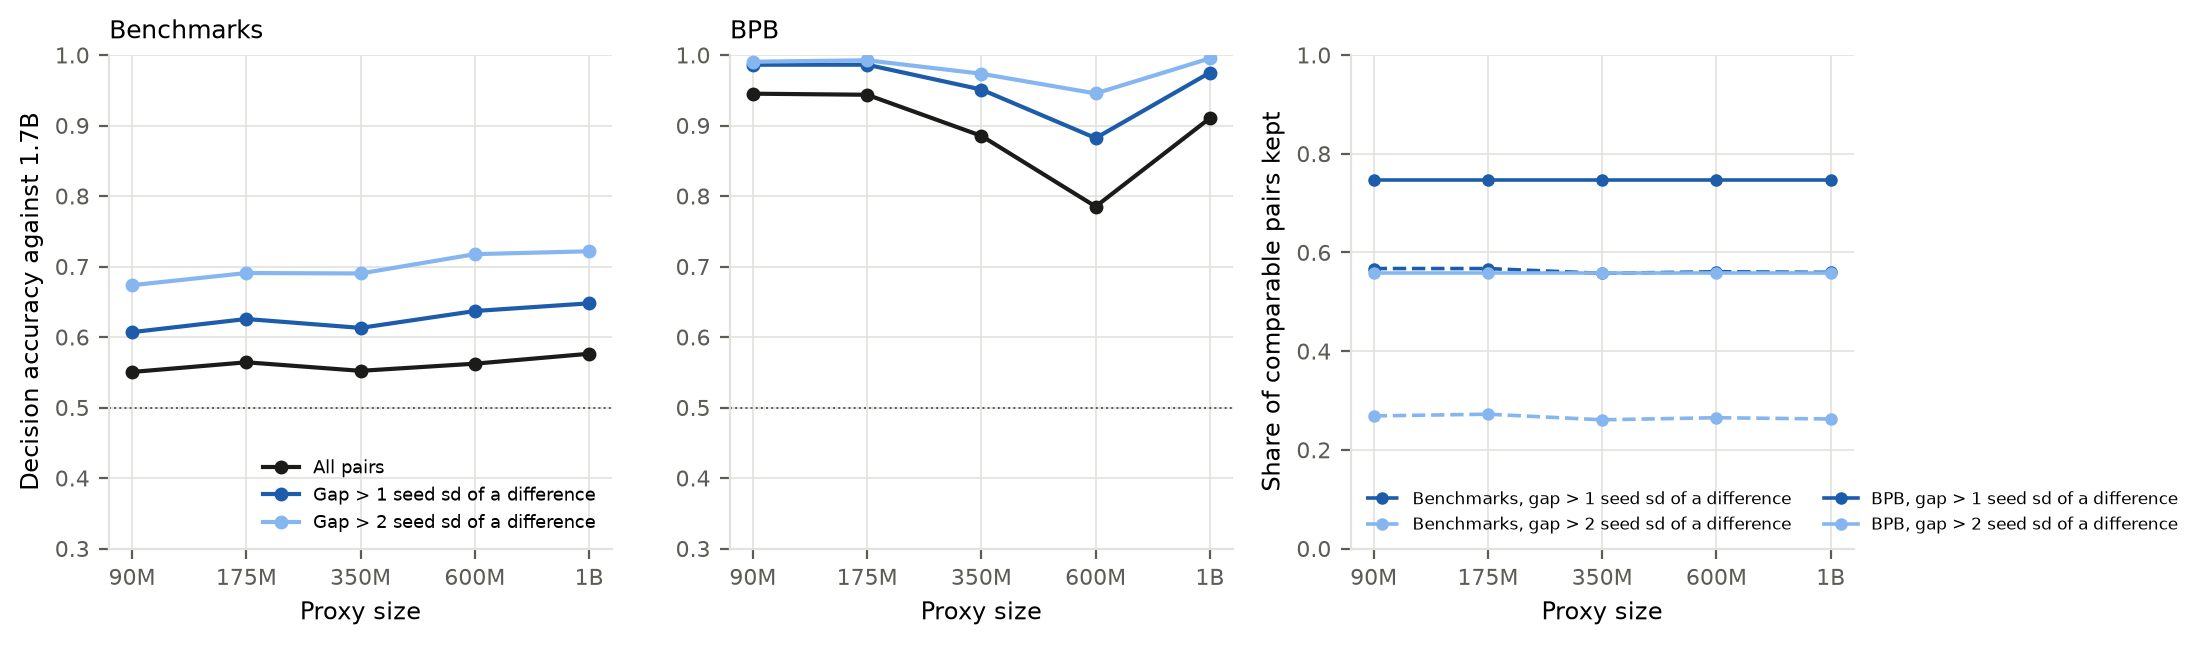
\includegraphics[width=\textwidth,height=0.36\textheight,keepaspectratio]{figures/app_rq02_decisive_pairs.png}
% source: src/signal-and-noise/analysis/rq02_decisive_pairs/pretraining/predictivity/decisive_pairs_da_size_paper.png
\captionof{figure}{\textbf{Benchmark DA rises on decisive pairs.} DA-size of the final checkpoint of each proxy size against the 1.7B final checkpoint, on multi-axis design pairs, for the benchmark tasks (left) and the per-language bits per byte (middle). One line per threshold: every comparable pair (black) and the pairs whose 1.7B gap exceeds one or two seed standard deviations of a difference (dark and light blue). The dotted line marks 0.5. Right: the share of the comparable pairs each threshold keeps, solid for the bits per byte and dashed for the benchmarks.}
\label{fig:app_rq02_decisive_pairs}
\end{minipage}
\vspace{\baselineskip}
}]
